\documentclass[10pt]{ctexbeamer}
\usepackage{bm}
\usepackage{tikz}
\usepackage{amsmath}
\usepackage{graphicx}
\newfontfamily{\dengxian}{DengXian}
\newCJKfontfamily{\fzyaoti}{FZYaoTi} %方正姚体
\newCJKfontfamily{\fzjinghong}{FZZJ-JHTJW} %方正字迹-惊鸿体
\newCJKfontfamily{\dqheiti}{Hiragino Sans GB} %冬青黑体
\newCJKfontfamily{\fandolhei}{FandolHei}

% \usetheme[color blocks]{Verona}% 使用Verona主题
% \usetheme[color blocks, red]{Verona}% 使用Verona主题, red theme
% \usetheme[color blocks, gray]{Verona}% 使用Verona主题, grey theme
\usefonttheme[onlymath]{serif}% 数学公式字体设置
\author{Norsesun}
\date{最后更新:\today}
\logo{
\includegraphics[height=1.2cm]{../../../Pngtree owl double exposure.png}}

\definecolor{airforceblue}{rgb}{.36,.54,.66}



\newcommand{\bmc}[1]{$\bm{#1}$}%定义一个新命令,行内数学模式的粗体,使幻灯片上的公式更清楚
\newcommand{\bmcc}[1]{
        \begin{displaymath}
            \bm{#1}
        \end{displaymath}
    }%定义一个新命令,行间数学模式的粗体,使幻灯片上的公式更清楚
\newcommand{\makecenter}[1]{\vspace{0.5em}\centering \parbox{.6\textwidth}{#1}}%定义一个新命令,居中排布一段话
\newenvironment{Mathbreakcenter}[1][1mm]{
        \par
        \vspace{#1} 
        \centering

    }{
        \par
        \vspace{2mm}
    }
\newcommand{\myblock}[3][1-]{
    \centering
    \begin{minipage}{.6\textwidth}
        \begin{block}<#1>{#2}%
            \centering%
            #3
        \end{block}
    \end{minipage}  
    } %定义一个新命令,居中排布一个block

    \newcommand{\myalertblock}[3][1-]{
        \centering
        \begin{minipage}{.6\textwidth}
            \begin{alertblock}<#1>{#2}%
                \centering%
                #3
            \end{alertblock}
        \end{minipage}  
        } %定义一个新命令,居中排布一个alertblock
\newcommand{\cleave}[2]{
    \hbox to #1{} #2 \hbox to #1{}
}
% \newcommand{\annmark}[1]{%
%     \textcolor{red}{$\bm\langle$#1$\bm\rangle$}%
% }%

% \newcommand{\ann}[1]{%
%     \begin{tikzpicture}[remember picture, baseline=-0.75ex]%
%         \node[coordinate] (inText) {};%
%     \end{tikzpicture}%
%     \marginpar{%
%         \renewcommand{\baselinestretch}{1.0}%
%         \begin{tikzpicture}[remember picture]%
%             \definecolor{orange}{rgb}{1,0.5,0}%
%             \draw node[fill=red!20,rounded corners,text width=\marginparwidth] (inNote){\footnotesize#1};%
%     \end{tikzpicture}%
%     }%
%     \begin{tikzpicture}[remember picture, overlay]%
%         \draw[draw = orange, thick]
%             ([yshift=-0.2cm] inText)
%                 -| ([xshift=-0.2cm] inNote.west)
%                 -| (inNote.west);%
%     \end{tikzpicture}%
% }%

% \setlength{\marginparwidth}{2.5cm}
% \renewcommand{\baselinestretch}{1.3}

\newenvironment{mathsalvation}[2][{解:}]{
    \begin{center}{}
        \begin{minipage}[t]{.05\textwidth}
            \vspace{0pt}
            {\color{#2}{#1}} \quad 
        \end{minipage}
        \begin{minipage}[t]{.7\textwidth}
            \vspace{0pt}
            % \fzyaoti
            % \dengxian
            % \fzjinghong
            % \dqheiti
            \fandolhei
}{
    \end{minipage}
    \end{center}
}

\usepackage{smartdiagram}

\title{解一元一次方程(1)}
\subtitle{Solve the Equation with one Unknown}

\AtBeginSubsection[\star]
{
	\begin{frame}{要点目录}
		\tableofcontents[currentsubsection]
	\end{frame}
}
\begin{document}
    \frame{\titlepage}

\section{合并同类项与移项}
\begin{frame}
    \centering
    \smartdiagramset{uniform color list=gray!90!black for 2 items,}
    \smartdiagram[priority descriptive diagram]{
        {能够从实际问题中列出一元一次方程,进一步体会\alert{方程模型思想}的作用及应用价值},
        {会利用\alert{合并同类项}的方法解一元一次方程,体会等式变形中的\alert{化归思想}}
    }
\end{frame}

\begin{frame}{合并同类项解一元一次方程}
    \makecenter{
        某校三年共购买计算机组140台,去年购买数量是前年的2倍,
        今年购买数量又是去年的2倍。前年这个学校购买了多少台计算机?
    }
    \myalertblock{1-}{}{
        \begin{enumerate}[<+->]
            \item 设未知数
            \item 找等量关系,列方程
            \item 合并同类项,解方程
        \end{enumerate}
    }
\end{frame}

\begin{frame}{温故知新}
    \begin{definition}
        含有相同的\alert{字母},并且相同字母的\alert{指数}也相同的项,叫做同类项。
    \end{definition}

    \begin{definition}
        合并同类项时,把各同类项的\alert{系数}相加减,字母和字母的指数\alert{不变}。
    \end{definition}
\end{frame}

\begin{frame}{用合并同类项化简}
    \makecenter{
        \begin{enumerate}
            \item \bmc{-3x+7x=}
            \item \bmc{\dfrac{1}{3}y+\dfrac{2}{3}y-2y=}
        \end{enumerate}
    }
\end{frame}

\begin{frame}{合并同类项}{尝试把一元一次方程转化成\bmc{x=m}(常数)的形式}
    \makecenter{\bmc{x+2x+4x=140}}
    \begin{figure}
        \includegraphics<2>[width=.7\textwidth]{assets/unite.png}
    \end{figure}
\end{frame}

\begin{frame}{合并同类项}{上述解方程中的“合并”起了什么作用?}
    \myalertblock{1}{}{
        解方程中“合并”起了化简作用,把含有未知数的项合并为一项,从而把方程转化为
        \bmc{ax = b}的形式,其中\bmc{a}、\bmc{b}是常数,“合并”的依据是\alert{逆用分配律}。
    }
\end{frame}

\begin{frame}{练习1}{利用合并同类项解简单的方程}
    \makecenter{\bmc{2x-\dfrac{5}{2}x=6-8}}

    \vspace{2em}

    \makecenter{\bmc{7x-2.5x+3x-1.5x=-15\times 4-6\times 3}}
\end{frame}

\begin{frame}{练习2}{利用合并同类项解简单的方程}
    \makecenter{\bmc{x-\dfrac{1}{2}x-\dfrac{1}{4}=15}}

    \vspace{2em}

    \makecenter{
        \bmc{|-x+\dfrac{2}{3}x+\dfrac{1}{2}x |=-4\times 2+ 3^2}}
\end{frame}

\begin{frame}{练习3}{列方程、解方程}
    \myblock{1-}{}{
        有一列数,按一定规律排列成1,-3,9,-27,81,
        -243 $\cdots$。 其中某三个相邻数的和是\bmc{-1701},这三个数各是
        多少?
    }
    \begin{figure}
        \includegraphics<2>[width=.55\textwidth]{assets/equation examp8.png}
    \end{figure}
\end{frame}

\begin{frame}{练习4}{列方程、合并同类项、解方程}
    \myblock{1-}{}{
        三个连续整数的和等于27,求这三个数。
    }
\end{frame}

\begin{frame}{练习5}{列方程解答实际问题}
    \begin{columns}
        \column{.7\textwidth}
        \begin{block}{}
            \centering%
            足球表面是由若干个黑色五边形和白色六边形皮块围成的,
            黑、白皮块数目的比为3:5,一个足球表面一共有32个皮块,
            黑色皮块和白色皮块
            各有多少个
        \end{block}

        \column{.25\textwidth}
        \begin{figure}
            
\includegraphics[width=.55\textwidth]{assets/2.png}
        \end{figure}
    \end{columns} 
    \begin{figure}
        \includegraphics<2>[width=.9\textwidth]{assets/3.png}
    \end{figure}
\end{frame}

\begin{frame}{归纳总结}
    \begin{figure}
        \includegraphics<1>[width=.95\textwidth]{assets/1.png}
    \end{figure}
\end{frame}

\begin{frame}{移项}
    \makecenter{解方程:\bmc{2x-\dfrac{5}{2}x=6-8}}

    \myalertblock{1}{}{
        观察下列一元一次方程,与上面的类型有什么区别?
        
        \bmc{3x +7 = 32-2x}
        }

        \vspace{1em}
        怎样才能使它向 \bmc{x=a }(\bmc{a}为常数)的形式转化呢?
\end{frame}

\begin{frame}{从等式性质1到移项}
    \myalertblock{1-}{}{
        把一些图书分给某班同学阅读,如果每人3本,则剩余20本;
        若每人4本,则还缺少25本,这个班的学生有多少人? 
    }

    \begin{figure}
        \includegraphics<2>[width=.8\textwidth]{assets/5.png}
    \end{figure}
\end{frame}

\begin{frame}
    \frametitle{移项的定义}
    \myalertblock{1}{}{
        一般地,把方程中的某些项改变符号后,
        从方程的一边移到另一边,这种变形叫做移项。 
    }

    \makecenter{移项实际上是利用等式的性质1。}
\end{frame}

\begin{frame}
    \frametitle{利用移项解一元一次方程}
    \myblock{1}{}{
        \bmc{3x+7=32-2x}
    }

    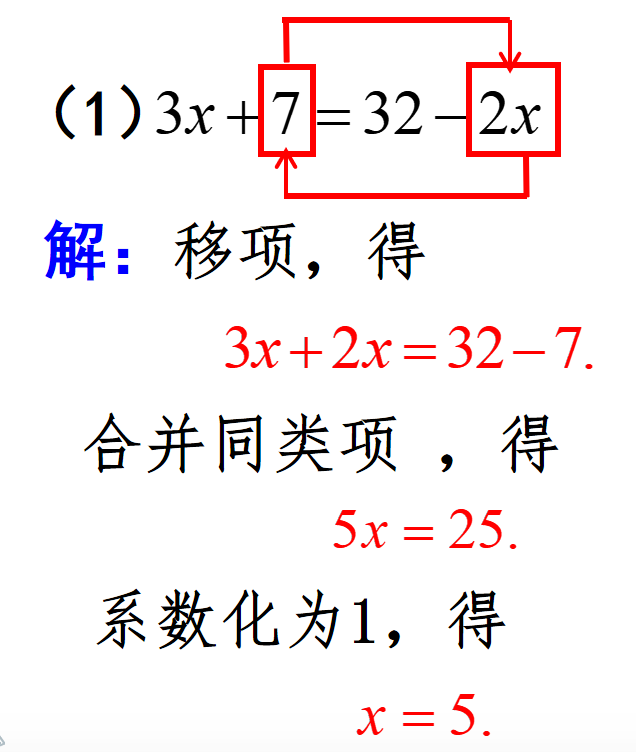
\includegraphics[width=.4\textwidth]{assets/7.png}
\end{frame}

\begin{frame}
    \frametitle{解一元一次方程的一般步骤}
    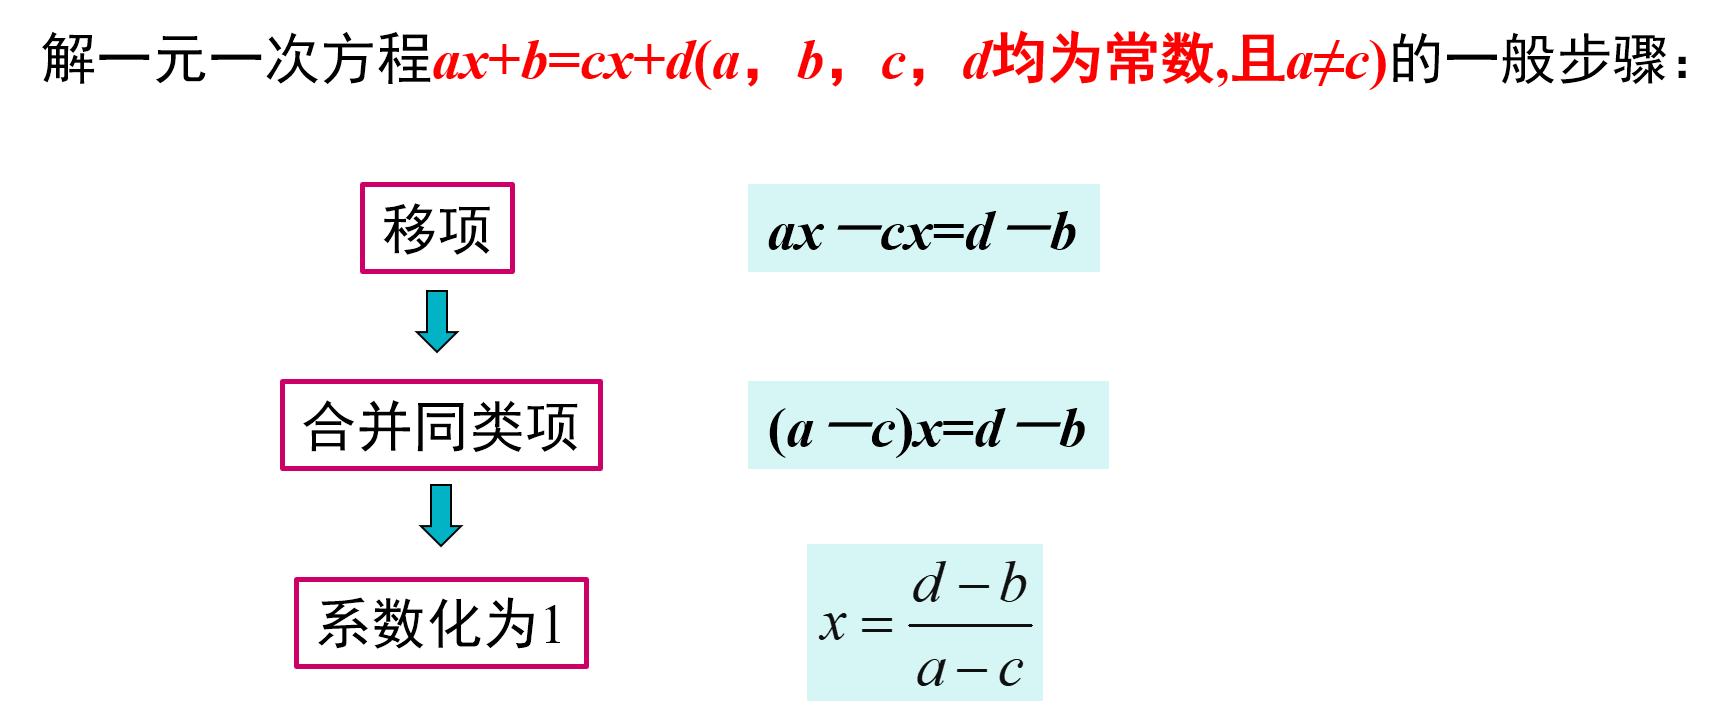
\includegraphics[width=.9\textwidth]{assets/8.png}
\end{frame}

\begin{frame}{练习5}{根据以下信息,你知道丢番图活了多少岁吗?}
    \begin{figure}
        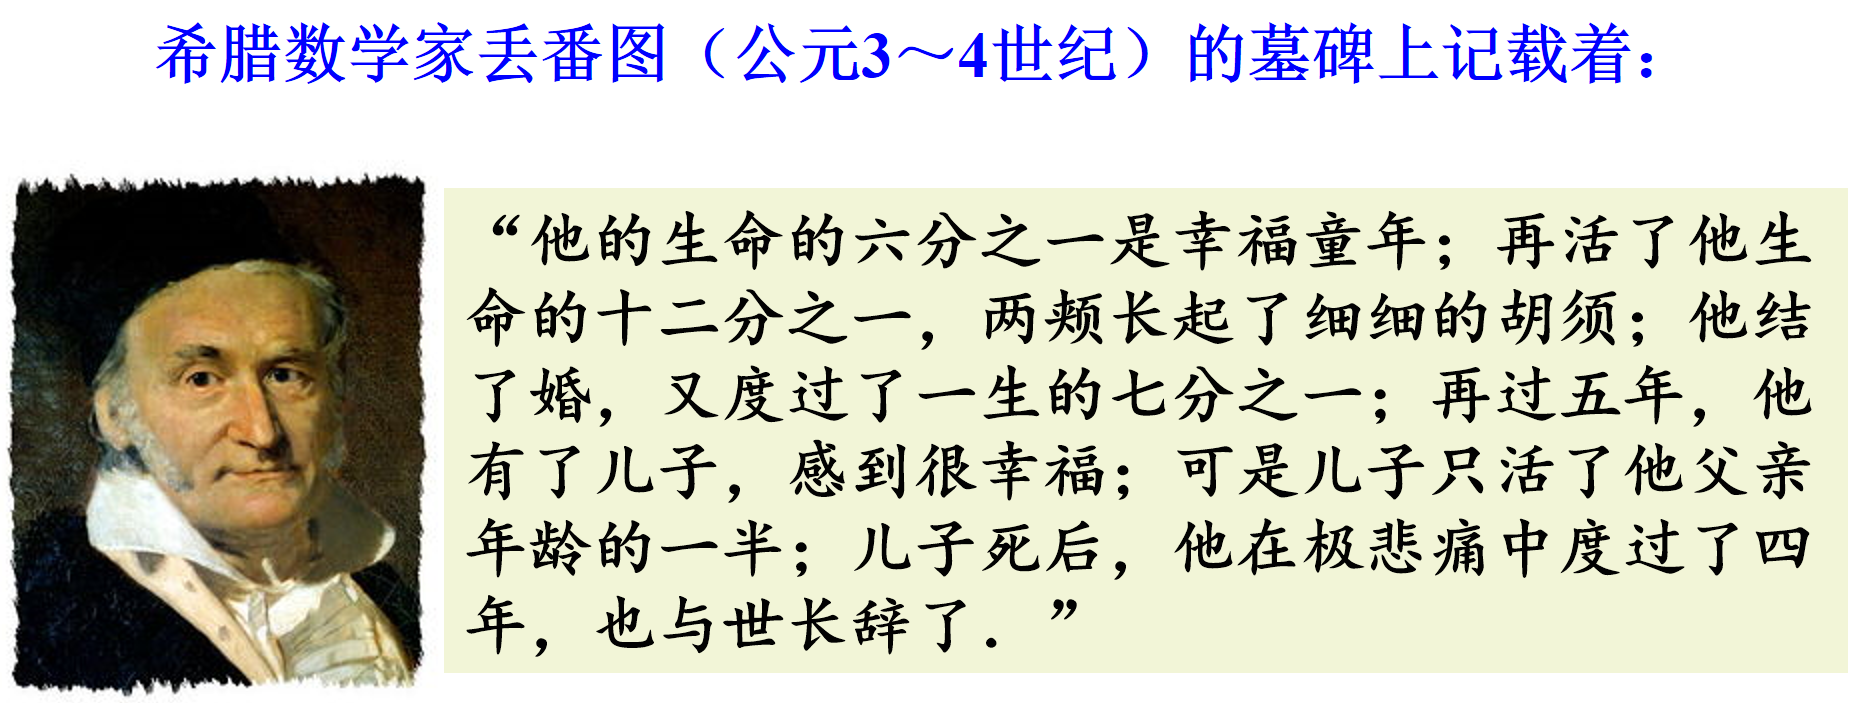
\includegraphics[width=.9\textwidth]{assets/4.png}
    \end{figure}
\end{frame}

\begin{frame}{练习6}{知识点:移项}
    \begin{figure}
        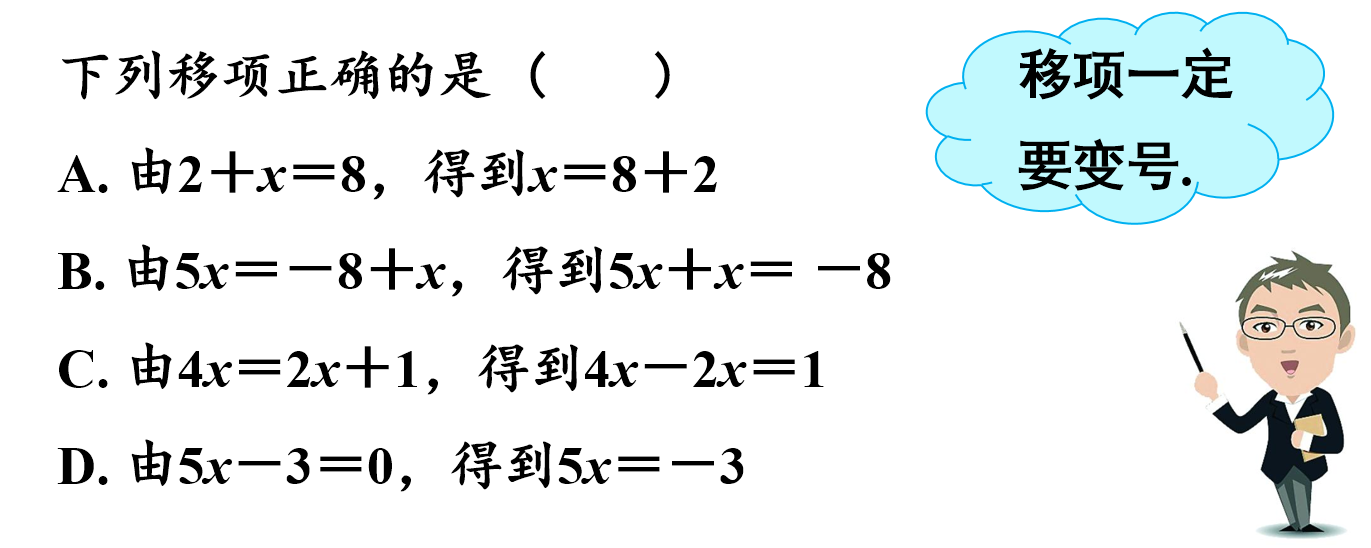
\includegraphics[width=.8\textwidth]{assets/6.png}
    \end{figure} 
\end{frame}

\begin{frame}{概览}
    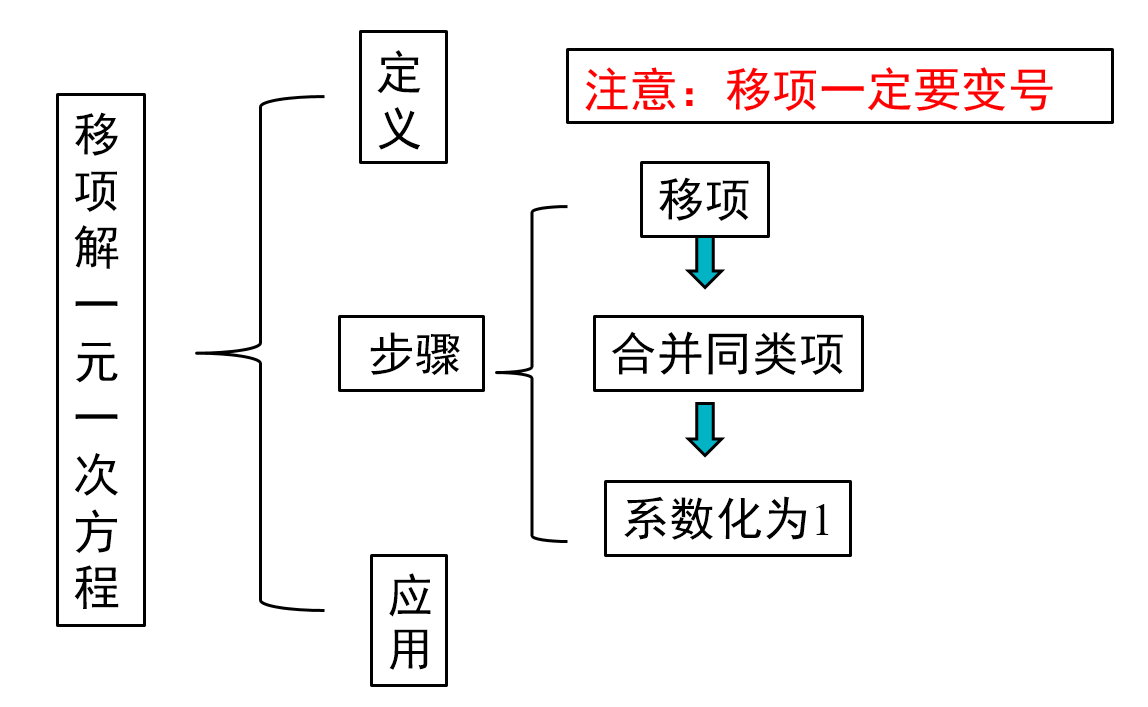
\includegraphics[width=.8\textwidth]{assets/10.png}
\end{frame}
\end{document}